\section{Allegorical model of rise run ruin rejuvenation}


I wanted to try to represent a certain style of stochastic cyclic dynamics. A pattern in which potential (energy) builds up constantly in the absence of use.  Then in surplus, the count of individual agencies (species) increases in response to the excessive energy potential. \par 
The potential is diminished by the large number of agencies until at some time,  a state of scarcity comes about. And in this, there is a catastrophic extinction in which all of the agencies die. In reality, not all of the agencies (species) will die, some will remain and become distinct in the newly hash selective conditions. \par 
From here, the cycle repeats. Potential once more begins to build until a Poission revival kickes off a new proliferative wave.  Yes, in reality, this will begin from one or a few of the agencies  remaining beyond the catastrophe. \par




\noindent
The purpose of this model is to make some link between a potential dynamics in the cyclic rise and decline of dissipative structures in the context of a constant supply of energy.  We perhaps see this style of dynamics both in the cyclic dynamics of turbulance shedding in the Stokes flow around a circle, and the periodic rise and collapse of ecosystems and even cultures. 

\subsection*{Model specification}

% Just notes, not final

(Energy availability)
 $$\ddt{N} = \xi - \mu \xt$$
(Segregation into multiplicity)
$$\pr{\Delta \xt = 1} = \lambda \xt \delt + o(\delt)$$
(Catastrophic collapse)
$$\pr{\xdt = 0 | \xt} =  \delta \frac{\xt}{N(t)} \delt +o(\delt)$$
(Poisson revival)
$$\pr{\xdt = 1 | \xt = 0} = \alpha \delt + o(\delt)$$
(No event)
$$\pr{\xdt = \xt} = 1 - \lrb{\lambda \xt  + \delta \frac{\xt}{N(t)} + \alpha   }\delt + o(\delt)$$



\begin{figure}[H]
    \centering
    % First figure
    \begin{subfigure}{0.48\textwidth}
        \centering
        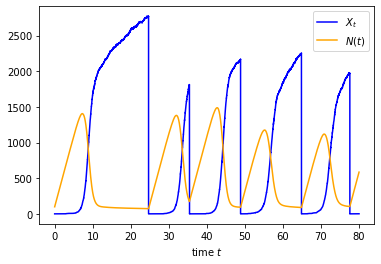
\includegraphics[width=\textwidth]{figures/IMG_ch8/VBCfigs/80for1VBC} % Adjust the image path as necessary
    \end{subfigure}
    \hspace{\fill} % Optional: adds space between figures
    % Second figure
    \begin{subfigure}{0.48\textwidth}
        \centering
        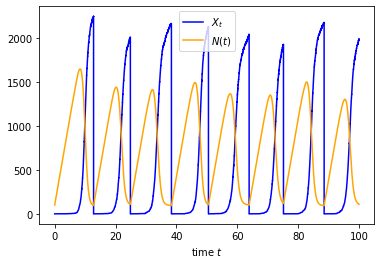
\includegraphics[width=\textwidth]{figures/IMG_ch8/VBCfigs/100for1VBC} % Adjust the image path as necessary
    \end{subfigure}
    
    \caption{Realisations of the model.  Potential energy, $N(t)$,  shown in orange, agency count,  $\xt$, in blue.}
    \label{fig:two_figures}
\end{figure}



\begin{figure}[H]
    \centering
    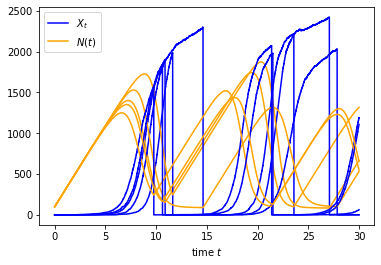
\includegraphics[width=0.7\textwidth]{figures/IMG_ch8/VBCfigs/30for5VBC} % Adjust the width as needed
    \caption{Multiple realisations with the same parameters and initial condition.}
    \label{fig:single_figure}
\end{figure}



\noindent
$\xt$, the replicative units (or objects of multiplicity in segregation) can be thought to represent a great many different things. They may be framed as the individuals in a population; of bacteria, viruses, organisms. They may be species within a genre, fractured but internally coherent groups within a broader population. Autonomous agencies within an organisation --- this is quite a general concept and could be applied to a number of situations: teams in a company, parties in a political system. A great many things can be placed in these terms... It would be fair to say that some of these representations are loose and ill-defined. But there is a more general way of looking at it, at what the quantity $\xt$ is attempting to capture. It's a proxy for order. That is, negative entropy. Think for a moment of a further analogy in fluid flows. If we observe the transition form laminar flow to turbulence, there is a fragmenting of flow directions. At first, all streamlines point in one onwards direction of motion. At the end of the transition, there are what appears to be an infinitude of ever more minute and fleeting divergences; of flow-lines separating off from one-another.\par



Admittedly, this does happen in spatial continuum rather than discrete jumps. But say for a moment we were to view this degenerative separation at a course grain. We might see from the outset an initial branching into two distinct pathways. Each of which encompassing fluid flow of roughly coherent direction. Each of these then has the potential to further subdivide into two. And each time this breakage takes place, there is further dissipation. In our coarse approximate description, there are a greater number of flow interfaces --- more locations of friction. Each sub-stream, smaller and smaller in cross-section will carry less and less kinetic energy and a greater proportion of the energy will be lost as heat.\par 
Towards the limit, minute, infinitely multiplicitous and scattered fluid trajectories will become so energy lacking as to resemble little more than stationary fluid. 
From here, with ongoing general flow, there will be a re-cohering into a more broadly aligned fluid stream. This, then, will likely be seen to once more progress in a dissipative turbulent divergence as before. In this way, a kind of oscillation commences. From Laminar, to turbulent, and through fizzling out, back to laminar, turbulent, so on and so forth. 

In real fluid flows --- take for example flow around a circle (or sphere in three dimensions) --- the oscillation is not absolute; both more turbulent and less turbulent regions coexist in an oscillatory spatial continuum. Laminar flow begins to shed turbulence as it sways one way in the wake of the circle; then going on to drift back into where the turbulence last was.\par 


Let us turn to another example of a dissipative structure: the fragmenting of a genus population into species over large swathes of time. That this is an example of a Prigoginian dissipative structure is a claim worth scrutinizing. I do believe it has been made before by others \cite{elitzur1994let} \cite{sharma2023assembly}.  None the less, let us be careful. 

Living organisms are one of the most rapidly dissipating arrangements in the universe. It has been observed that per kilogram, humans and other terrestrial life forms dissipate energy as a rate orders of magnitude greater than the sun. They are also highly ordered, local low-entropy formations which are kept far above equilibrium by their continual usage of energy. So it seems natural to assign the term ``dissipative structure'' to living organisms taken at the individual level. 
But can we speak more generally about life and its natural progressions? Over time, genera fragment into species. It seems straightforward that this is an example of entropy reduction.  



\vspace{10pt}

\hrule

\vspace{10pt}



\noindent
\textbf{Aside:} In "The genetical theory of natural selection" (1930),  R.  Fisher makes mentions something in relation to this line of thought: 

\begin{quote}
\noindent
"A philospohical view of history, which has attained to great popularity in several continental countries,  regards the rise as well as the fall of civilisations as but successive phases of a cycle of growth and decay,  which, it is supposed, repeats itself endlessly,  throughout human history.  So long as we aim at no more than an effective generalised description of the phenomena there is much to be said for considering the phases of rise and development of the great civilisations in conjunction with the phases of their decayand collapse. It is a real advantage that the parallelisms between the earlier phases of different cultures should be recognised, and that their relations in time to recognizably parallel later phases should be established as accurately as possible.  Generalised description should, however,  never be regarded as an aim in itself."
\end{quote}

"Generalised description should, however,  never be regarded as an aim in itself" -- maybe I should have read this before working on the equations above.  But perhaps there is a certain utility in the aesthetic of a generalised description when it becomes codified in the language of a mathematical model. 




\vspace{10pt}

\hrule


\vspace{10pt}
